\section{Method}
\label{sec:method}

This section gives the complete QCert methodology: formalization of the false-alarm contract (Section~\ref{sec:contract}), a fixed-point deployment arithmetic model (Section~\ref{sec:arith}), the three mechanisms by which quantization breaks decisions together with a falsifiable error bound (Section~\ref{sec:mechanisms}), a division-free integer decision layer that holds by construction (Section~\ref{sec:decision-layer}), integer quantile estimation (Section~\ref{sec:int-quantile}), zero-data threshold transport (Section~\ref{sec:transport}), and the overall static pipeline (Section~\ref{sec:pipeline}).
The whole chapter revolves around one central thesis: \emph{calibrating the threshold in floating point while inferring in fixed point is a silently failing paradigm error; this paper moves the false-alarm contract into integer arithmetic so that it holds by construction on the deployed graph.}

\subsection{The false-alarm contract and notation}
\label{sec:contract}

\subsubsection{Decision statistic and contract}
\label{sec:contract-def}

Let the input SAR scene be $x$. The detector $f_\theta$ outputs a per-position score field $s(u)\in\mathbb{R}$ (the raw logit passed through sigmoid, or its inverse transform), where $u$ is a spatial position.
Introduce the per-position first- and second-order statistics $(\mu(u),\sigma(u))$ given by a null model, and define the standardized decision statistic
\begin{equation}
z(u) \;=\; \frac{s(u)-\mu(u)}{\max\!\big(\sigma(u),\,\varepsilon\big)},\qquad \varepsilon>0 .
\label{eq:z}
\end{equation}
On the clutter-location set $\OmC(x)$ (no true targets; construction in Section~\ref{sec:three-sets}), take the $1-\alpha$ quantile as the per-scene threshold
\begin{equation}
\lambda(x) \;=\; \mathrm{Quantile}_{1-\alpha}\Big(\{\,z(u):\,u\in\OmC(x)\,\}\Big),
\label{eq:lambda-scene}
\end{equation}
with decision rule
\begin{equation}
\hat{y}(u) \;=\; \mathbb{1}\{\,z(u)>\lambda(x)\,\}.
\label{eq:decision}
\end{equation}

Equation~\eqref{eq:lambda-scene} gives the threshold of the \textbf{per-scene mode}.
In parallel there is the \textbf{global mode}: merge the clutter locations of all calibration scenes into a mixed pool and take a single threshold
\begin{equation}
\lambda_{\mathrm{glob}} \;=\; \mathrm{Quantile}_{1-\alpha}\Big(\bigcup_{x\in\mathcal{X}_{\mathrm{cal}}}\big\{\,z(u):\,u\in\OmC(x)\,\big\}\Big),
\tag{3.2a}
\label{eq:lambda-glob}
\end{equation}
replacing $\lambda(x)$ in Eq.~\eqref{eq:decision} by $\lambda_{\mathrm{glob}}$ at decision time.
The two modes share the same contract framework but optimize different objectives and cannot both be attained; see Table~\ref{tab:modes}.

\begin{table}[htbp]
\centering
\caption{Two operating points of the same contract.}
\label{tab:modes}
\small
\begin{tabular}{p{2.2cm}p{1.6cm}p{1.9cm}p{4.1cm}p{4.3cm}}
\toprule
Mode & Calibration pool & $\ncal$ scale & Advantage & Cost \\
\midrule
Global (Eq.~\eqref{eq:lambda-glob}) & cross-scene mixed & large ($\sim10^{5}$) & smallest calibration error of $\mathbb{E}[\Pfa]$ (E9: err 0.0185 dex) & conditional false-alarm rate varies with scene --- rough-sea $\Pfa(x)>\alpha$, candidate load degrades with sea state (E7) \\
Per-scene (Eq.~\eqref{eq:lambda-scene}) & single scene & small ($\sim4\times10^{3}$) & $\Pfa(x)\approx\alpha$ per scene; candidate load $\approx\alpha\,n_{\mathrm{cell}}$ decoupled from sea state (E7) & large calibration variance (E9: err 0.201 dex), and constrained by the lower bound $\alpha\ge 1/(\ncal+1)$ \\
\bottomrule
\end{tabular}
\end{table}

The two modes are two legal operating points of the same contract: latency/expectation-sensitive links take the global mode, while load/tail-latency-sensitive links take the per-scene mode.
The load-suppression claim of E7 uses the per-scene mode and the accuracy claims of E8/E9 use the global mode; each is labeled at its own place and they must not be read together.

The measured pixel-level false-alarm rate is
\begin{equation}
\Pfa^{\mathrm{pixel}} \;=\; \frac{\#\{\,u\in\Omega:\,\hat{y}(u)=1\,\}}{|\Omega|},
\label{eq:pfa}
\end{equation}
where $\Omega$ is a measurement set constructed independently of $\OmC$.
Equation~\eqref{eq:pfa} is the \textbf{false-alarm contract}.
Its statistical meaning must be stated precisely --- it is not the hard guarantee ``$\Pfa\le\alpha$ for every scene'' (impossible under finite samples), but
\begin{equation}
\mathbb{E}[\Pfa]=\alpha,\qquad
\mathrm{Var}(\Pfa)\le \frac{\alpha(1-\alpha)}{\neff+1},
\label{eq:contract}
\end{equation}
where $\ncal$ is the total number of clutter positions entering calibration and $\neff$ is the effective number of independent blocks folded in by block sampling (see Section~\ref{sec:three-sets}).
Three points must be stated honestly:

\textbf{(i) The expectation equality only needs exchangeability, not independence.}
For exchangeable sequences, the rank argument on order statistics gives $\mathbb{E}[\Pfa]=\alpha$ exactly; spatial correlation does not break the expectation, it only inflates the variance --- the $\neff$ in the variance bound is precisely the fold-in of correlation.
Reachable nominal levels have a lower bound $\alpha\ge 1/(\ncal+1)$: our per-scene calibration has $\ncal\approx4\times10^{3}$ (clutter cells per scene), giving a lower bound $\sim2\times10^{-4}$, so $\alpha=10^{-3}$ is reachable; when the block-sampling keep ratio drops, $\ncal$ shrinks in step --- at keep$=1/16$, $\ncal\approx5\times10^{2}$ and the lower bound rises to $\sim2\times10^{-3}>\alpha$, where the contract is not reachable in the first place, and E9's measured $\Pfa=4.7\times10^{-3}$ at that level is pressed exactly to the $1/\ncal$ scale (Table~\ref{tab:e9a}) --- a direct confirmation of the lower bound, not an anomaly.

\textbf{(ii) The contract controls fluctuation, not bias.}
The expectation in Eq.~\eqref{eq:contract} is taken with respect to the calibration distribution; the discipline of Section~\ref{sec:three-sets} requires the measurement set $\Omega$ to be constructed differently from $\OmC$, and the systematic distribution shift between them appears as a fixed bias of $\mathbb{E}[\Pfa]$ relative to $\alpha$, outside the coverage of the rank-statistic bound.
We expose it honestly through the deviation $D$ (Eq.~\eqref{eq:deviation}): in E0, the pooled $\Pfa=1.60\times10^{-3}$ of FP16 itself deviates from $\alpha$ by about 60\% (due to construction differences between calibration and measurement), unrelated to quantization ($R=0.969$).
The contract promises ``fluctuations around the reachable operating point are bounded''; the bias of the operating point itself is exposed by $D$, not hidden.

\textbf{(iii) Acceptance convention.}
Engineering acceptance measures contract keeping by $|\log_{10}(\Pfa/\alpha)|$, referenced against the calibration noise floor (the residual deviation after a full re-calibration on the same data; see Sections~\ref{sec:e5}/\ref{sec:e9}); all calibration results are reported together with $\ncal$ and $\neff$, not the nominal $n$ alone.

\subsubsection{Primary metric: the accuracy-invariance ratio}
\label{sec:R-def}

Our core observable is not mAP but the \textbf{accuracy-invariance ratio}
\begin{equation}
R \;=\; \frac{\Pfa^{\,\mathrm{INT8}}}{\Pfa^{\,\mathrm{FP32}}},
\qquad
|\log_{10} R| \;\text{is the reported quantity},
\label{eq:R}
\end{equation}
and the \textbf{contract deviation}
\begin{equation}
D \;=\; \left|\log_{10}\frac{\Pfa^{\,\mathrm{INT8}}}{\alpha}\right|
\;\xrightarrow{\text{across sea states}}\; D_{\max}=\max_{\text{bucket}}\,D .
\label{eq:deviation}
\end{equation}
The $R$ criterion has two tiers, used uniformly throughout:

\begin{itemize}
\item \textbf{Existence gate} $R\ge 1.5$: a degradation of the false-alarm rate by more than $1.5\times$ counts as hard evidence that ``silent failure exists'' (used by E0). $R\approx1$ or $R<1$ means no degradation is observed, judged NO-GO --- \textbf{this does not mean the method fails; it means the failure does not exist under this configuration}, and the audit reports the negative honestly.
\item \textbf{Invariance band} $|\log_{10}R|\le 0.176$ (i.e.\ $R\in[0.67,\,1.5]$): the acceptance band for contract equivalence across quantization (E8 uses the stricter $R\le1.2$). All claims of transport/decision-layer pass if $R$ falls inside the invariance band and the deviation $|D|$ does not exceed the calibration noise floor.
\end{itemize}

\subsubsection{Three sets that must stay disjoint (guarding against circular reasoning)}
\label{sec:three-sets}

\begin{table}[htbp]
\centering
\caption{The three sets that must be constructed disjointly.}
\label{tab:three-sets}
\small
\begin{tabular}{p{3.2cm}p{4.4cm}p{2.4cm}p{4.2cm}}
\toprule
Set & Construction & Use & Forbidden \\
\midrule
Quantization calibration set $C_{\mathrm{quant}}$ & $\ge64$ real SAR images per sea state (stratified) & AMCT determines scale/range & using calm seas only (shrinks range $\to$ saturation) \\
Contract calibration set $\OmC$ & clutter locations after dilating GT boxes by a guard band of $g$ px, plus target-free tiles, block-sampled & compute $\lambda(x)$ & using in-box pixels \\
Measurement set $\Omega$ & constructed differently from $\OmC$ & report $\Pfa$ & overlapping $\OmC$ \\
\bottomrule
\end{tabular}
\end{table}

Block sampling partitions $\OmC$ into $B\times B$ blocks ($B=64$ px) and samples whole blocks with ratio $k$, mitigating inflated effective sample sizes caused by spatial correlation:
\begin{equation}
\neff \;=\; \frac{|\Omega|}{B^{2}}\cdot k .
\label{eq:neff}
\end{equation}

\emph{Key distinction.} AMCT uses \emph{images} to choose ranges, while we use \emph{clutter locations} to choose quantiles --- the two optimize different quantities. This distinction is itself a finding of this paper.

\subsection{Fixed-point deployment arithmetic model and three assumptions}
\label{sec:arith}

\subsubsection{Per-layer affine int8 model}
\label{sec:affine}

The detector $f_\theta$ and the null model are compiled into \textbf{one single static graph}, whose activations are per-layer affine int8 quantized:
\begin{equation}
a_q \;=\; \mathrm{clamp}\!\Big(\mathrm{round}\!\big(\tfrac{a}{\Delta_l}\big)+z_l,\,-128,\,127\Big),
\label{eq:affine}
\end{equation}
where $\Delta_l$ (scale) and $z_l$ (zero-point) are the quantization parameters of layer $l$, \textbf{fixed at compile time and readable}.
Dequantization is $\hat{a}=\Delta_l\,(a_q-z_l)$.
For the single-family output heads (three detection heads $\mathrm{cv3}.\{0,1,2\}$), the quantization step is aggregated into a scalar by a cell-count-weighted geometric mean (see Section~\ref{sec:head-agg}).

\subsubsection{Three explicit assumptions}
\label{sec:assumptions}

All conclusions of this paper rest on the following three assumptions, which must be stated explicitly:
\begin{itemize}
\item \textbf{A1 (same-device bit reproducibility)}: the same .om is bit-reproducible on the same device (integer kernel determinism). This is the foundation of ``thermal steady state does not affect $\Pfa$'' and of ``the transport rule is definable''.
\item \textbf{A2 (cross-implementation inconsistency)}: across devices or quantization configurations, int8 outputs are not guaranteed to agree (different kernel accumulation orders $\to$ different rounding $\to$ different tail orderings).
\item \textbf{A3 (readable quantization configuration)}: per-layer $(\Delta_l,z_l)$ and the output ranges are readable by the user (AMCT/ATC artifacts).
\end{itemize}
Under A1--A3, this paper claims: \textbf{the false-alarm contract can hold by construction in integer arithmetic, and is covered by the analytic bound in the A2 case.}

\subsubsection{Deployment instantiation: what $\mu$, $\sigma$ are in our SSDD chain}
\label{sec:null-inst}

The $\mu(u),\sigma(u)$ of Eq.~\eqref{eq:z} form a general framework (any per-position null model applies), and their instantiation must be stated explicitly, otherwise the integer codes $\mu_q,\sigma_q$ of the decision layer are undefined.
We distinguish two levels:
\begin{itemize}
\item \textbf{General framework}: $\mu(u),\sigma(u)$ are per-position null-model statistics (e.g.\ local clutter mean/standard deviation), affine-quantized like $s$ (Eq.~\eqref{eq:affine}) into integer codes $\mu_q,\sigma_q$. The synthetic audit experiments (E1/E4 and the synthetic items of E9) adopt this full form.
\item \textbf{Our SSDD deployment instance (used by all board-level experiments)}: the raw-logit score field of the detector serves \emph{directly} as the decision statistic, i.e.\ the degenerate case
\begin{equation}
\mu(u)\equiv 0,\qquad \sigma(u)\equiv \sigma_{0}\ \ (\text{fixed constant}).
\tag{3.9a}
\label{eq:null-degenerate}
\end{equation}
Then $\mu_q\equiv0$ and $\sigma_q\equiv\mathrm{round}(\sigma_0/\Delta_\sigma)$ are compile-time constants; $\Delta_\sigma$ is a \textbf{normalization grid chosen by the decision layer itself} ($1/128$ in this paper, see Section~\ref{sec:head-agg}) --- a design parameter, not a PTQ product.
Substituting into Eq.~\eqref{eq:z}, $z(u)=s(u)/\sigma_0$, and the quantile threshold $\lambda$ together with $\sigma_0$ is absorbed into $\lambda_{int}$ (Section~\ref{sec:transport}); the decision degenerates to ``score field $>$ integer threshold''.
\end{itemize}

\textbf{Two consequences must be stated honestly:}
\begin{enumerate}
\item \textbf{The denominator mechanism ($\varepsilon_\sigma$ term) of Section~\ref{sec:mech-denom} does not act in our deployment instance} --- $\sigma$ is a fixed constant, so there is no quantization error of $\sigma$.
That mechanism is the dominant threat for the more general null-model deployments with per-position $\sigma$, covered by the synthetic experiments E1/E4; in our SSDD instance the dominant threat is the \textbf{output-grid mechanism} ($\Delta_s$, Section~\ref{sec:mech-grid}), exactly consistent with the E5 measurement (when $\Delta_s$ changes by $10\times$, the no-conversion drift is 300$\times$).
\item The rationale for choosing the logit as the decision statistic: after BCE training the logit tail is approximately monotone in clutter strength, so its quantile threshold is a ``pixel-level CFAR-like'' threshold; we do not claim the logit is the optimal null-model statistic, and the generalization to per-position $\mu/\sigma$ is left as future work.
\end{enumerate}

\subsubsection{Why mAP cannot see this problem}
\label{sec:map-blind}

mAP integrates over the ranking of all detections and is insensitive to the 99.9th percentile; yet $\Pfa=\alpha=10^{-3}$ is determined by exactly that percentile.
Hence a wide interval exists:
\begin{equation}
\big|\Delta\,\mathrm{mAP}\big|<1\ \text{point}\quad\not\Longrightarrow\quad R\approx 1 ,
\tag{3.10}
\label{eq:map-blind}
\end{equation}
i.e.\ mAP barely moves while $\Pfa$ can change severalfold.
\textbf{This is the gap this paper occupies} --- all existing PTQ research optimizes mAP.

\subsection{Three mechanisms by which quantization breaks decisions, and an error bound (C1 theory)}
\label{sec:mechanisms}

Let the quantization perturbations be $\hat{s}=s+e_s$, $\hat{\mu}=\mu+e_\mu$, $\hat{\sigma}=\sigma+e_\sigma$, with
\begin{equation}
|e_s|\le\tfrac{\Delta_s}{2},\qquad |e_\mu|\le\tfrac{\Delta_\mu}{2},\qquad |e_\sigma|\le\tfrac{\Delta_\sigma}{2}.
\label{eq:errors}
\end{equation}

\subsubsection{Mechanism 1: the denominator mechanism (dominant for general null-model deployments; inactive in our SSDD instance)}
\label{sec:mech-denom}

\emph{Applicability statement}: this mechanism requires $\sigma(u)$ to be a per-position quantity participating in quantization.
In our SSDD deployment instance $\sigma$ is a fixed constant (Section~\ref{sec:null-inst}), so this error source does not exist; the mechanism targets more general null-model deployments with per-position $\sigma$, whose numerical verification is carried by the synthetic experiments E1/E4.

A first-order expansion of Eq.~\eqref{eq:z} gives
\begin{equation}
\hat{z}-z \;\approx\; \frac{e_s-e_\mu-z\,e_\sigma}{\sigma}.
\label{eq:first-order}
\end{equation}
When $z$ is moderately large (and decisions care exactly about the tail), the $z\,e_\sigma$ term dominates.
Defining the \textbf{measured quantization-step ratio}
\begin{equation}
\varepsilon_\sigma \;=\; \frac{\Delta_\sigma}{2\sigma},
\label{eq:eps-sigma}
\end{equation}
we have $\hat z-z\approx -z\,\varepsilon_\sigma$.
For the Gaussian upper tail $\Pfa(z)=1-\Phi(z)$, from $\mathrm{d}\ln(1-\Phi)/\mathrm{d}z=-\phi/(1-\Phi)\approx-(z+1/z)$ we get
\begin{equation}
\ln\frac{\Pfa(\hat z)}{\Pfa(z)} \;\approx\; z^{2}\,\varepsilon_\sigma .
\label{eq:scale-law}
\end{equation}

Equation~\eqref{eq:scale-law} is the most important first-order prediction of this paper: \textbf{false-alarm drift amplifies with $z^2$ and linearly with $\varepsilon_\sigma$}.
At $\alpha=10^{-3}$ ($z\approx 3.09$, $z^2\approx 9.55$) --- a first-order upper-bound scale; E1 measures $1/2$--$1/24$ of the prediction, so the bound is conservative, see Section~\ref{sec:e1} --- Table~\ref{tab:eps-scan} quantifies the amplification.

\begin{table}[htbp]
\centering
\caption{Amplification of $\Pfa$ by null-scale quantization error at $\alpha=10^{-3}$ (first-order upper-bound scale).}
\label{tab:eps-scan}
\small
\begin{tabular}{lcc}
\toprule
$\varepsilon_\sigma$ & $\ln$ multiple $z^2\varepsilon_\sigma$ & $\Pfa$ multiple $e^{z^2\varepsilon_\sigma}$ (upper-bound scale) \\
\midrule
2\%  & 0.19 & $\times$1.21 \\
5\%  & 0.48 & $\times$1.63 \\
10\% & 0.95 & $\times$2.65 \\
20\% & 1.91 & $\times$7.0 \\
\bottomrule
\end{tabular}
\end{table}

\emph{Corollary (under the general framework).} In deployments with per-position $\sigma$, the quantization granularity of $\sigma$ is the primary contradiction, not the precision of $s$.
This suggests two designs: (i) parameterize $\sigma$ in the log domain; (ii) \textbf{eliminate division} in the decision (Section~\ref{sec:decision-layer}).

\emph{Correction of the corollary (stated honestly).} The synthetic ablation E4 shows that log-domain/per-channel $\sigma$ brings only $\le1.85\times$ improvement, short of the predicted $\ge5\times$ (P1 fails, Section~\ref{sec:e4}).
We therefore downgrade ``the $\sigma$ term dominates'' to a \textbf{first-order scaling law} ($\Delta\ln \Pfa\sim\varepsilon_\sigma^{\,2}$, measured exponent $1.96\approx2$, holds) plus a \textbf{conservative empirical bound} (Proposition~\ref{prop:bound}, holds), and no longer claim that improving the $\sigma$ granularity yields an order-of-magnitude gain.
In our SSDD deployment instance $\sigma$ is fixed (Section~\ref{sec:null-inst}), so the corollary does not apply directly.

\subsubsection{Mechanism 2: output saturation (fixed-point only)}
\label{sec:mech-sat}

The output range of the score head comes from calibration-set statistics.
In high-clutter scenes, strong echoes push $s$ against the int8 upper bound, and many positions receive the same maximal integer --- a \textbf{tie}:
\begin{equation}
\text{tie}\;\Rightarrow\;\text{ranking information lost}\;\Rightarrow\;\lambda\ \text{pushed to the bound}\;\Rightarrow\; \Pfa\ \text{explodes or}\ P_d\ \text{collapses}.
\label{eq:tie}
\end{equation}
This mechanism does not exist under FP16 and \textbf{can only be observed and audited on a fixed-point graph}.
Define the per-layer saturation rate
\begin{equation}
\mathrm{sat}_l \;=\; \frac{\#\{a_q=127\ \text{or}\ -128\}}{\#\text{elements}},
\label{eq:sat}
\end{equation}
reported per layer $\times$ per sea state, together with the number of ties within the top $1\%$ of the score field --- direct evidence of ``ranking collapse''.

\emph{Countermeasure}: the range calibration set must be stratified by sea state ($\ge64$ images in each of the three buckets); $\sigma$ and $s$ get separate ranges and never share.

\subsubsection{Mechanism 3: output grid and per-layer rounding (dominant in our SSDD instance; the root of cross-device non-portability)}
\label{sec:mech-grid}

Output-grid mechanism: the score head output lands on a lattice of compile-time step $\Delta_s$ (this also holds for FP16 --- its raw logits lie exactly on the piecewise-uniform fp16 lattice, with $\mathrm{ulp}=2^{-7}$ on the main segment, see Section~\ref{sec:head-agg}).
The threshold $\lambda$ must land on the same grid, otherwise the decision shifts on the lattice and $\Pfa$ jumps accordingly.
\textbf{This is the dominant threat of our deployment instance (fixed $\sigma$)}: changing the quantization configuration changes $\Delta_s$, and an old threshold misaligns on the new grid.

Superimposed on this is accumulated per-layer rounding:
\begin{equation}
|e_s| \;\le\; \sum_{l}\frac{\Delta_l}{2}\,\kappa_l,
\label{eq:rounding}
\end{equation}
where $\kappa_l$ is the gain from layer $l$ to the output.
In practice this effect is much smaller than the denominator mechanism, but it is the root of \textbf{cross-device non-portability} (A2): different kernels accumulate in different orders $\to$ different rounding $\to$ different tail orderings.
This is exactly why ``transport'' rather than ``recompute'' is necessary across configurations.

\subsubsection{Proposition 2 (false-alarm deviation bound)}
\label{sec:prop2}

\begin{proposition}
\label{prop:bound}
Let $\Pfa(z)=1-F_z(z)$ have Lipschitz constant $L$ on $[\lambda-\delta,\lambda+\delta]$. Then
\begin{equation}
\big|\,\Pfa(\hat z)-\Pfa(z)\,\big| \;\le\; L\cdot\delta,
\qquad
\delta \;=\; \frac{\Delta_s/2+\Delta_\mu/2+\lambda\,\Delta_\sigma/2}{\sigma}.
\tag{3.18}
\label{eq:bound}
\end{equation}
\end{proposition}

\textbf{Operational form}: $\delta$ is \textbf{computed entirely from the scale tables} (no new data needed); $L$ uses the analytic density in synthetic audits (where the distribution is known) and \textbf{only the empirical density of the calibration set $\OmC$} in real deployments --- using the measurement set $\Omega$ to estimate $L$ is strictly forbidden, as it would be ``validating test data with test data'' (the discipline of Section~\ref{sec:three-sets} applies here as well).

\textbf{First-order approximation} (the Proposition~\ref{prop:bound} form of Eq.~\eqref{eq:scale-law}):
\begin{equation}
\Delta\ln \Pfa\;\approx\;z^{2}\,\varepsilon_\sigma .
\tag{3.19}
\label{eq:bound-first-order}
\end{equation}

\textbf{Falsifiable prediction (P1)}: after switching $\sigma$ to a log-domain parameterization plus per-channel scales, the measured $\Delta\ln \Pfa$ should drop by $\ge 5\times$.
If P1 fails, the ``$\sigma$ term dominates'' claim of Proposition~\ref{prop:bound} needs revision --- we report this honestly in Section~\ref{sec:e4}.

\subsection{Division-free integer decision layer (C2 system)}
\label{sec:decision-layer}

\subsubsection{Division elimination (core)}
\label{sec:divfree}

In general $s/\mu/\sigma$ come from three different layers with different scales ($\Delta_s,\Delta_\mu,\Delta_\sigma$).
Multiplying both sides of the decision $(s-\mu)/\sigma>\lambda$ by $\sigma\cdot 2^{K}/\Delta_s$ ($K$ is a fixed-point shift; 64-bit intermediates eliminate truncation) yields a \textbf{purely integer comparison}:
\begin{equation}
\boxed{\;
\hat{y}(u)=\mathbb{1}\Big\{\,
\underbrace{s_q(u)\,2^{K}}_{\text{shift}}\;-\;
\underbrace{\Big(\tfrac{\Delta_\mu}{\Delta_s}2^{K}\Big)\,\mu_q(u)}_{\text{compile-time const.}\,\cdot\,\text{integer}}
\;>\;
\underbrace{\Big(\lambda\,\tfrac{\Delta_\sigma}{\Delta_s}2^{K}\Big)}_{\text{compile-time constant}}\,
\max\!\big(\sigma_q(u),\sigma_{\min}\big)\,\Big\}}
\tag{3.20}
\label{eq:int-decision-full}
\end{equation}
Writing $b=\mathrm{round}(\frac{\Delta_\mu}{\Delta_s}2^{K})$, $c=\mathrm{round}(\lambda\frac{\Delta_\sigma}{\Delta_s}2^{K})$, $r=2^{K}$, this is
\begin{equation}
\underbrace{r\,s_q - b\,\mu_q}_{\text{LHS (int64)}} \;>\;
\underbrace{c\,\max(\sigma_q,\sigma_{\min})}_{\text{RHS (int64)}}.
\tag{3.21}
\label{eq:int-decision}
\end{equation}

\textbf{Special case} ($\Delta_s=\Delta_\mu$; in this paper $s$ and $\mu$ come from the same source): letting $d_q=(s_q-\mu_q)\ll k$, the decision simplifies to
\begin{equation}
d_q \;>\; \lambda_{int}\cdot\max(\sigma_q,\sigma_{\min}),
\qquad
\lambda_{int}=\mathrm{round}\!\Big(\lambda\,\tfrac{\Delta_\sigma}{\Delta_s}\,2^{k}\Big).
\tag{3.22}
\label{eq:int-decision-simple}
\end{equation}

\textbf{Properties}: all-integer multiply-add, no division, no floating point, no quantization of $z$; $2^{K}$ and $\lambda_{int}$ are fixed at compile time $\Rightarrow$ \textbf{the graph can be fully staticized}.

\begin{lemma}[Decision equivalence]
\label{lem:equivalence}
With int64 intermediates, the integer decision of Eq.~\eqref{eq:int-decision} agrees position-by-position with the FP32 decision $\hat y=\mathbb{1}\{(s-\mu)/\max(\sigma,\sigma_{\min})>\lambda\}$ on the quantization lattice; the only differences come from (i) the rounding of $b,c$ ($\le 2^{-K}$ relative error), and (ii) the quantization of $\sigma_q,\mu_q,s_q$ (covered by the bound of Proposition~\ref{prop:bound}).
\end{lemma}

\begin{proof}[Proof sketch]
Substitute $\hat s=\Delta_s s_q$, $\hat\mu=\Delta_\mu\mu_q$, $\hat\sigma=\Delta_\sigma\sigma_q$ into the FP32 decision and multiply both sides by $\sigma 2^K/\Delta_s>0$ (the inequality direction is preserved); LHS$-$RHS is integer-valued.
With int64, none of $r s_q$, $b\mu_q$, $c\sigma_q$ overflows ($K=20$, $|s_q|,|\mu_q|,|\sigma_q|\le 2^{31}$, $|b|,|c|\le 2^{K+1}$, products $\le 2^{53}$), hence no truncation error and the equivalence holds.
\end{proof}

\subsubsection{Integer quantiles ($O(B)$, no sorting)}
\label{sec:int-quantile}

The key observation for calibrating $\lambda$: \textbf{a quantile needs counting, not sorting}.
\begin{enumerate}
\item Compute $d_q(u)=(s_q-\mu_q)\cdot 2^{k}$ on the NPU (or in host integer code);
\item histogram into $B$ buckets (4096 here), indexed by the high bits of $d_q$;
\item prefix-sum to locate the bucket containing the $m=\lceil(n+1)(1-\alpha)\rceil$-th sample;
\item linear interpolation within the bucket yields $\lambda_{int}$.
\end{enumerate}

\textbf{Bucket width vs finite-sample error}: quantile localization has two error terms --- the bucket-width term ($\le$ bucket width $W$) and the finite-sample term.
The complete $\alpha$ error bound is
\begin{equation}
|\Delta\alpha|\;\le\;\underbrace{\frac{1}{B}}_{\text{bucket width}}\;+\;\underbrace{O\!\Big(\sqrt{\tfrac{\alpha}{\neff}}\Big)}_{\text{finite sample}},
\tag{3.23}
\label{eq:quantile-err}
\end{equation}
where the second term usually dominates: at $B=4096$ the bucket-width term is $2.4\times10^{-4}$, yet E9 measures an $\alpha$ error of $8.4\%$ ($\neff\approx50$), fully explained by $\neff$ (Section~\ref{sec:e9}).
Hence ``$<10^{-4}$ after interpolation'' holds only when $\neff$ is large enough; we report both terms honestly and no longer quote the bucket-width bound alone.
This makes ``per-scene calibration'' an $O(n)$ single pass on a 1~GHz CPU/NPU instead of $O(n\log n)$.

\subsubsection{Host-free and bit-exact}
\label{sec:hostfree}

\begin{itemize}
\item The decision graph and the detection graph are fused into a single .om; the host only does DMA and logging;
\item repeated runs of the same .om agree bit by bit (A1; measured bit-exact rate 1.0 in Section~\ref{sec:e3});
\item cross-implementation differences are acknowledged by A2 and covered by the bound of Proposition~\ref{prop:bound}.
\end{itemize}

\subsection{Integer-domain calibration (preferred path)}
\label{sec:int-calib}

The stronger practice is \textbf{not to transport at all}: compute the quantile of $\OmC$ directly in the integer domain (Section~\ref{sec:int-quantile}); then $\lambda$ lives in the same domain as inference and the contract holds by construction.
Reconstruct the floating-point $z$ from integer codes (for diagnostics/calibration only):
\begin{equation}
\tilde z(u)=\frac{\Delta_s\,s_q(u)-\Delta_\mu\,\mu_q(u)}{\max(\Delta_\sigma\,\sigma_q(u),\,\varepsilon)},
\qquad
\lambda=\mathrm{Quantile}_{1-\alpha}\big(\{\tilde z(u):u\in\OmC\}\big).
\tag{3.24}
\label{eq:int-calib}
\end{equation}
The transport rule of Section~\ref{sec:transport} is reserved for cases where re-calibration cannot be re-run (zero-data migration across sensors).

\subsection{Zero-data threshold transport (C1 system)}
\label{sec:transport}

\subsubsection{The transport rule (a pure function of two scale tables)}
\label{sec:transport-rule}

Floating-point threshold $\lambda$ ($z$ domain) $\to$ integer threshold under a given configuration:
\begin{equation}
\lambda_{int} \;=\; \mathrm{round}\!\Big(\lambda\cdot\frac{\Delta_\sigma}{\Delta_s}\cdot 2^{k}\Big).
\tag{3.25}
\label{eq:transport-int}
\end{equation}
Given an old integer threshold $\lambda_{int}^{old}$ (old configuration $(\Delta_s^{old},\Delta_\sigma^{old})$), moving to a new configuration $(\Delta_s^{new},\Delta_\sigma^{new})$ only needs
\begin{equation}
\boxed{\;
\lambda_{int}^{new} \;=\; \mathrm{round}\!\Big(
\lambda_{int}^{old}\cdot
\frac{\Delta_\sigma^{new}}{\Delta_\sigma^{old}}\cdot
\frac{\Delta_s^{old}}{\Delta_s^{new}}\Big)\;}
\tag{3.26}
\label{eq:transport}
\end{equation}
with the inverse transform (for diagnostics):
\begin{equation}
\lambda \;=\; \frac{\lambda_{int}\,\Delta_s}{\Delta_\sigma\,2^{k}} .
\tag{3.27}
\label{eq:transport-inv}
\end{equation}

\textbf{This is what ``zero-data'' means}: when changing the quantization configuration, the calibration set, or the device, one only reads out the new scales and recomputes a single integer $\lambda_{int}$ --- \textbf{no re-run of the calibration set}.
This is precisely a capability that ``only this kind of board can provide'': the rule is a \textbf{pure-function mapping between integer lattices}, whose existence requires the conjunction of A1 (bit-reproducibility on the lattice) and A3 (scales readable at compile time).
A floating-point GPU pipeline has no global lattice carrying the decision threshold (kernel accumulation order is determined at runtime); even though explicit-QDQ frameworks (TensorRT/TFLite) also export scale tables, ``rounding the threshold onto the lattice'' is undefined in floating point --- \textbf{the transport rule is therefore \emph{undefinable} on floating-point GPUs, not merely inconvenient.}

\textbf{Degenerate form in the deployment instance} (our SSDD chain, fixed $\sigma$): $\Delta_\sigma$ does not change across configurations (Section~\ref{sec:null-inst}) $\Rightarrow$ the ratio $\Delta_\sigma^{new}/\Delta_\sigma^{old}=1$ in Eq.~\eqref{eq:transport}, and transport simplifies to
\begin{equation}
\lambda_{int}^{new}\;=\;\mathrm{round}\!\Big(\lambda_{int}^{old}\cdot\frac{\Delta_s^{old}}{\Delta_s^{new}}\Big),
\tag{3.26a}
\label{eq:transport-degenerate}
\end{equation}
i.e.\ the integer threshold is transported \emph{inversely} to the output-grid step.
Equation~\eqref{eq:transport-degenerate} is the form used by all E5 measurements.

\textbf{$\Delta_s$ on the FP16 side}: FP16 is not ``unquantized'' --- the raw logits lie exactly on the piecewise-uniform fp16 lattice, and the measured cells of the main segment $[-16,-8)$ have $\mathrm{ulp}=2^{-7}=0.0078125$ (probe residuals all zero).
Hence FP16$\to$INT8 transport equally applies Eq.~\eqref{eq:transport-degenerate} with $\Delta_s^{old}$ taken as this ulp.
This is the definitional basis of E5 setting 2.

\subsubsection{Output-head step aggregation}
\label{sec:head-agg}

For the three output heads $\mathrm{cv3}.\{0,1,2\}$ (cell counts $80^2/40^2/20^2=6400/1600/400$ at 640 input), the scalar step is the cell-count-weighted geometric mean:
\begin{equation}
\Delta_s \;=\; \exp\!\Big(\frac{\sum_{l=0}^{2} w_l\,\ln d_l}{\sum_l w_l}\Big),
\qquad (w_0,w_1,w_2)=(6400,1600,400),
\tag{3.28}
\label{eq:head-agg}
\end{equation}
where $d_l$ is the quantization step of head $\mathrm{cv3}.l.2$.
$\Delta_\sigma$ takes the decision-layer $\sigma$ grid ($1/128$ here, \textbf{a design constant chosen by the decision layer, outside PTQ scope, not changing with model configuration}).

\subsubsection{First-order transport error}
\label{sec:transport-error}

The extra $z$-domain deviation introduced by transport comes from \textbf{lattice rounding} (the residual of round in Eqs.~\eqref{eq:transport-int}/\eqref{eq:transport}, transformed back to the $z$ domain via Eq.~\eqref{eq:transport-inv}):
\begin{equation*}
|\Delta z_{\mathrm{transport}}| \;\le\; \frac{\Delta_s}{2\,\Delta_\sigma\, 2^{k}} .
\end{equation*}
With $\mathrm{d}\ln \Pfa/\mathrm{d}z \approx -(z+1/z)$ (Section~\ref{sec:mech-denom}), the first-order transport error is given per case.

\textbf{General null-model deployment} (per-position $\sigma$ quantized; Mechanism 1 of Section~\ref{sec:mech-denom}): the \emph{configuration-dependent part} of the $\sigma$-rounding bias $z^2\varepsilon_\sigma$ becomes residual error after transport, superimposed on the lattice-rounding term:
\begin{equation}
\big|\Delta\ln \Pfa^{\,\mathrm{transport}}\big|
\;\lesssim\;
\underbrace{z^{2}\,\big|\varepsilon_\sigma^{\mathrm{new}}-\varepsilon_\sigma^{\mathrm{old}}\big|}_{\text{cross-config.\ difference of the $\sigma$-rounding bias}}
\;+\;
\underbrace{(z+1/z)\,\frac{\Delta_s}{2\,\Delta_\sigma\, 2^{k}}}_{\text{lattice rounding}} .
\tag{3.29}
\label{eq:transport-err-general}
\end{equation}

\textbf{Degenerate form for the deployment instance} (our SSDD chain: $\sigma\equiv\sigma_0$ fixed, $\Delta_\sigma=1/128$ a design constant of the decision layer; neither changes with configuration): $\varepsilon_\sigma^{\mathrm{new}}=\varepsilon_\sigma^{\mathrm{old}}$, and the first term of Eq.~\eqref{eq:transport-err-general} is \textbf{identically zero} --- the residual bias of $\sigma$ rounding has already been absorbed in integer-domain calibration (calibration runs on the real integer pipeline, Section~\ref{sec:int-calib}; whatever residual remains is identical for both configurations and cancels in cross-configuration transport), so it is not a transport error:
\begin{equation}
\big|\Delta\ln \Pfa^{\,\mathrm{transport}}\big|
\;\lesssim\;(z+1/z)\,\frac{\Delta_s}{2\,\Delta_\sigma\, 2^{k}}
\;\approx\;z\,\frac{\Delta_s}{2\,\Delta_\sigma\, 2^{k}} .
\tag{3.29a}
\label{eq:transport-err-degenerate}
\end{equation}

Hence in the SSDD instance the transport error reduces to the single lattice-rounding term, fully controlled by the design parameter $2^{k}$ (make $2^k$ large and the error is arbitrarily small).
This is consistent with the applicability statement of Section~\ref{sec:mech-denom}: the denominator mechanism is inactive in the SSDD instance, so the first term of Eq.~\eqref{eq:transport-err-general} never appears; the transport accuracy of the SSDD instance is measured by E5 (Section~\ref{sec:e5}).

\subsection{Overall static pipeline}
\label{sec:pipeline}

The complete deployment pipeline (cf.\ Fig.~\ref{fig:pipeline}):

\begin{figure}[htbp]
\centering
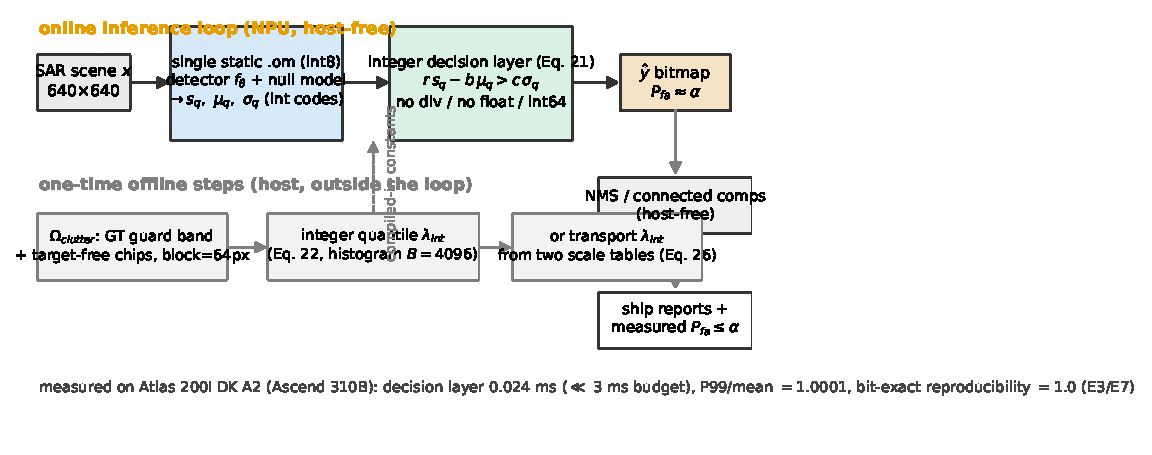
\includegraphics[width=0.86\linewidth]{figs/fig2_pipeline.pdf}
\caption{The QCert static deployment pipeline. The detector and null model are compiled into one static .om (int8, A3-readable scales); the integer decision layer (Eq.~\eqref{eq:int-decision}) fuses decision and inference into the same graph, so the host only performs DMA. Offline one-shot steps: $\OmC$ construction and integer-quantile calibration/transport of $\lambda_{int}$.}
\label{fig:pipeline}
\end{figure}

\textbf{One-shot offline steps} (host, outside the inference loop): (i) $\OmC$ construction; (ii) integer-quantile calibration of $\lambda_{int}$ (Eq.~\eqref{eq:int-decision-simple}) or transport (Eq.~\eqref{eq:transport}).
The inference loop runs entirely on the NPU and the host exits $\Rightarrow$ decision-layer cost $\ll 3$ ms (measured $0.024$ ms, see Section~\ref{sec:e7}).

\subsection{Method summary}
\label{sec:method-summary}

\begin{table}[htbp]
\centering
\caption{Method components at a glance.}
\label{tab:method-summary}
\small
\begin{tabular}{p{2.6cm}p{1.7cm}p{5.0cm}p{3.6cm}}
\toprule
Component & Equation & Role & Irreplaceability \\
\midrule
Contract & \eqref{eq:pfa}\eqref{eq:contract} & defines $\mathbb{E}[\Pfa]=\alpha$ (in expectation) and the lower bound $\alpha\ge1/(\ncal+1)$ & distinguishes from mAP optimization \\
Dual-mode threshold & \eqref{eq:lambda-scene}\eqref{eq:lambda-glob} & global for expected accuracy / per-scene for load equalization & two operating points of one contract \\
Denominator mechanism & \eqref{eq:eps-sigma}\eqref{eq:scale-law} & $\Delta\ln \Pfa\approx z^2\varepsilon_\sigma$ (general null-model deployments) & guides design; inapplicable to the SSDD instance \\
Prop.~\ref{prop:bound} & \eqref{eq:bound} & closed-form error bound; $\delta$ from scale tables & distinguishes from engineering tuning \\
Integer decision & \eqref{eq:int-decision}\eqref{eq:int-decision-simple} & division-free, sort-free, host-free, bit-exact & unique to fixed-point boards \\
Integer quantile & \eqref{eq:quantile-err} & $O(n)$ sort-free calibration & per-scene feasible \\
Threshold transport & \eqref{eq:transport} & zero-data across configurations/sensors & \textbf{no lattice on floating-point GPUs; undefinable} \\
\bottomrule
\end{tabular}
\end{table}
